\documentclass[../../Aurora C# unofficial manual.tex]{subfiles}

\begin{document}
	\section{Setting ground formation support}
	Original post can be found
	\href{http://aurora2.pentarch.org/index.php?topic=8495.msg109807#msg109807}{here}.
	\\\\
	
	Here is a screenshot of the UI for setting support relationships between superior and subordinate formations. You drag the superior formation on to the subordinate formation. If the Support checkbox is checked, the supporting formation is shown in blue-grey with the name of the supported formation. Any supported formation in shown in orange. Support can only be provided when the supporting formation is a superior formation in the hierarchy of the supported formation, or is directly subordinate to a superior formation in the hierarchy of the supported formation and does not itself have any subordinate formations (an independent artillery formation for example). Supporting formations must be on the same system body as the supported formation. In combat, the support relationship will only function if the supporting unit has suitable bombardment units and is in a support or rear echelon position and the supported unit is in a front line position.
	
	The drag-drop is intelligent and can distinguish between setting support relationships, reassigning formations to a new headquarters, removing headquarters assignments, moving formations from one population to another (on the same system body) and moving elements between formations (more on that last option in section \ref{ground_formation_element_transfer_ui}).
	\begin{figure}[H]
		\centering
		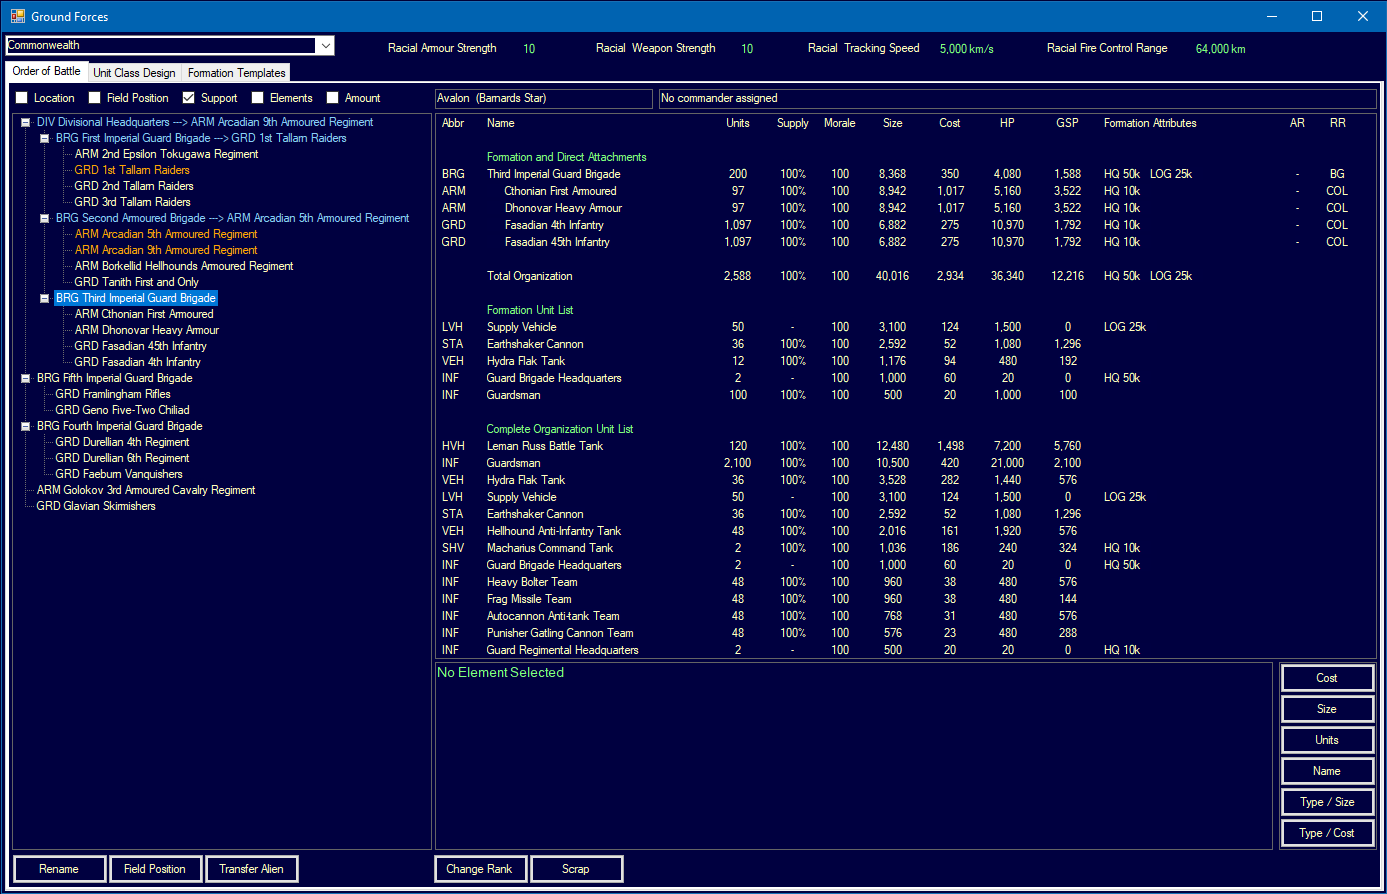
\includegraphics[width=0.95\linewidth]{images/GroundFormationSupport}
		\caption[Ground Formation Support]{Ground Formation Support Example}
		\label{fig:groundformationsupport}
	\end{figure}
\end{document}